\maketitle
\setcounter{page}{1}
\tableofcontents
\newpage
\pagenumbering{arabic}
\section{Theorie}
\subsection{Berechnung der Beugungsbildes durch Interferenz}
Ziel des Versuchs ist die Betrachtung der $\textsc{Frauenhofer}$-Lichtbeugung an Parallel- und
Doppelspalten.
Optische Beugung tritt immer dann auf, wenn Licht auf ein Objekt trifft, dessen
Abmessungen kleiner sind, als der Durchmesser des Lichtstrahls selbst. Zur Erklärung
von Beugungsphänomenen muss zuerst unterschieden werden, ob die Lichtquelle im endlichen liegt und der
Lichtstrahl auseinander läuft, oder ob die Lichtquelle so weit von der Beugungsebene
entfernt liegt, dass der Lichtstrahl als paralleles Bündel auftrifft. Es wird dann
davon gesprochen, dass die Lichtquelle "ins Unendliche verschoben wurde". Der erste Fall wird
als $\textsc{Fresnel}$-Beugung bezeichnet, der Zweite als $\textsc{Frauenhofer}$-Beugung
(siehe Abbildung \ref{abb:1}).
\begin{figure}
  \centering
  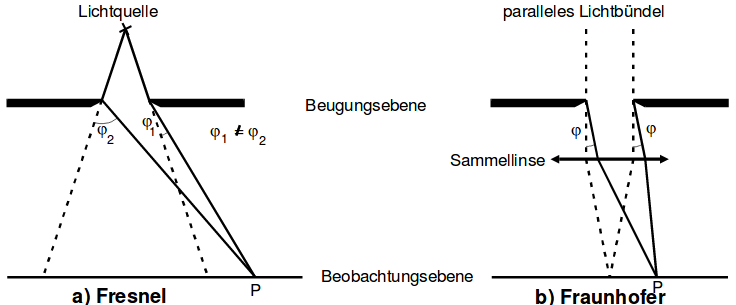
\includegraphics[scale=0.4]{fresfrau.png}
  \caption{Veranschaulichung der $\textsc{Fresnel}$- und $\textsc{Frauenhofer}$-Beugung \cite{anleitung}.}
  \label{abb:1}
\end{figure}
Die theoretisch einfacher zu erklärende $\textsc{Frauenhofer}$-Beugung wird hier am Parallelspalt diskutiert. Es gelten
folgende Annahmen.
\begin{itemize}
  \item Die Spaltbreite ist gering gegenüber der Spaltlänge, sodass der Strahl nur in
  seiner Breite begrenzt wird.
  \item Es werden nur Strahlen betrachtet, die unter dem selben Winkel gebeugt wurden.
  Um dies zu realisieren, muss der Abstand zwischen Beobachtungsebene groß im Vergleich
  mit der Spaltbreite sein. Dafür wird häufig eine Sammellinse in den Strahlengang nach
  der Beugungebene gebracht.
  \item Es treffen ebene Wellen der Form
  \begin{equation}
    A(z,t) = A_0 \exp \left ( \symup{i} \left(\omega t - \frac{2 \pi z}{\lambda}\right) \right)
    \label{eq:1}
  \end{equation}
  mit Wellenlänge $\lambda$ auf die Beugungsebene auf. Um dies zu realisieren ist
  kohärentes Licht notwendig, dass "aus dem Unendlichen" kommend auf den Spalt trifft.
  Als Quelle solchen Lichtes werden beispielsweise Laser genutzt.
\end{itemize}
Alle Punkte der eintreffenden Wellenfront sind nun nach dem $\textsc{Huygens}$schen
Prinzip Ausgangspunkt einer sich kugelförmig ausbreitenden Elementarwelle. Trifft der
Strahl auf den Spalt führt dies dazu, dass der Lichtstrahlen in Teilstrahlen
aufgeteilt wird, die untereinander interferieren, da es einen Gangunterschied $s$ zwischen ihnen
gibt (siehe Abbildung \ref{abb:2}) Aus diesem Gangunterschied lässt sich eine Phasenunterschied
$\delta$ betimmen:
\begin{equation}
  \delta = \frac{2 \pi s}{\lambda} = \frac{2 \pi x \sin(\varphi)}{\lambda}.
  \label{eq:2}
\end{equation}
Aus \eqref{eq:1} und \eqref{eq:2} lässt sich nun ein Ausdruck für die Amplitude $B$
in Abhängigkeit des Winkels finden:
\begin{equation}
  B(\varphi) = A_0 b \, \symup{sinc}(\eta)
  \label{eq:3}
\end{equation}
mit
\begin{equation}
  \eta = \frac{\pi b \sin(\varphi)}{\lambda}.
\end{equation}
Die Amplitude ist jedoch nicht messbar, da die Frequenz des Lichtes extrem hoch
und daher für Messgeräte nicht auflösbar ist. Messbar ist jedoch die Intensität,
die dem Quadrat der Amplitudenfunktion entspricht:
\begin{equation}
  I(\varphi) \propto B(\varphi)^2 = A_0^2 b^2 \, \symup{sinc}^2(\eta).
  \label{eq:4}
\end{equation}
Diese Funktion wird auch als Beugungsfigur bezeichnet.
\begin{figure}
\centering
  \begin{subfigure}{0.3\textwidth}
    \centering
    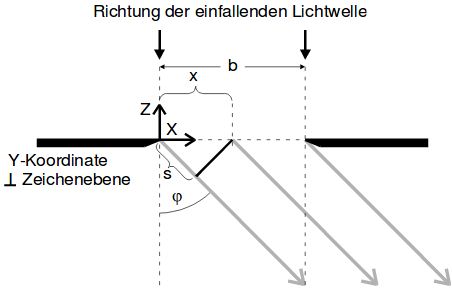
\includegraphics[width=\textwidth]{einzel.png}
    \caption{Einzelspalt \cite{anleitung}.}
    \label{abb:2}
  \end{subfigure}
  \begin{subfigure}{0.6\textwidth}
    \centering
    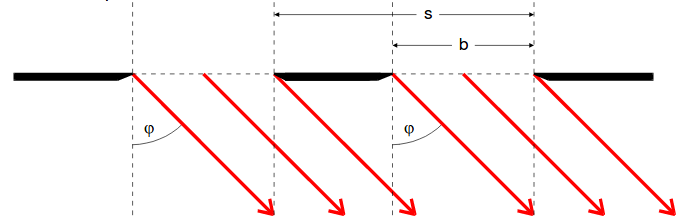
\includegraphics[width=\textwidth]{doppel.png}
    \caption{Doppelspalt \cite{anleitung}.}
    \label{abb:3}
  \end{subfigure}
  \caption{Veranschaulichung der Interferenzeffekte an Einzel- und Doppelspalt}
\end{figure}
Wie für den Einzelspalt lässt sich eine Beugungsfigur auch für den Doppelspalt definieren.
Hier muss jedoch der Gangunterschied $s$ anders definiert werden (siehe Abbildung \ref{abb:3}).
Man erhält:
\begin{equation}
  B(\varphi)^2 = A_0 \cos^2\left(\frac{\pi s \sin(\varphi)}{\lambda} \right) \, \symup{sinc}^2(\eta).
  \label{eq:5}
\end{equation}
Aufgrund der großen Abstände zwischen Photoelement und Beugungsebene lässt
sich sowohl für den Einzel- als auch für den Doppelspalt der Winkel $\varphi$
in guter Näherung durch
\begin{equation}
  \varphi \approx \tan(\varphi) = \frac{x - x_0}{L}
  \label{eq:6}
\end{equation}
bestimmen. $L$ ist dabei der Abstand zwischen Spalt und Photoelementebene, $x_0$ die Position
des Maximums 0. Ordnung und $\symup{\Delta}x$ der Abstand zwischen $x_0$ und dem
betrachteten Punkt.
\subsection{Berechnung des Beugungsbildes durch Fourier-Transformation}
Die Intensitätsfunktion kann auch aus der Fourier-Transformierten der sogenannten
Aperturfunktion, also jener Funktion die das Objekt, an dem gebeugt wird, beschreibt,
bestimmt werden. Die Aperturfunktion ist dabei für alle $x$ der beugenden Geometrie
gleich der Amplitude $A_0$ (also beispielsweise zwischen den Begrenzungen eines Spaltes),
ansonsten ist sie null. Die Fourier-Transformationsformel
\begin{equation}
  g(\xi) = \int_{-\infty}^\infty f(x) \exp(\symup{i} x \xi)
  \label{eq:7}
\end{equation}
liefert dann mit der Aperturfunktion $f(x)$ das Beugungsbild. Rücktransformation liefert
entsprechend die Geometrie des Objektes.
\section{Durchführung}
\subsection{Versuchsaufbau}
Der Versuchsaufbau (siehe Abbildung \ref{abb:4}) besteht aus einer optischen Bank
auf der ein Laser, eine Halterung mit Spaltplatten und ein Photoelement befestigt werden.
Das Photoelement ist dabei auf einer Schiene befestigt, auf der es über eine Milimeterschraube
quer zur optischen Bank verschoben werden kann. Als Laser wird ein Helium-Neon-Laser
mit einer Wellenlänge von $\lambda \approx \SI{633}{\nano\metre}$ genutzt. Es stehen
Spaltplatten mit verschiedenen Einzel- und Doppelspalten zur Auswahl. Das Photoelement
ist an ein Amperemeter mit einem Messbereich in Größenordnungen zwischen \num{e-3}
und \SI{e-9}{\ampere} angeschlossen.
\begin{figure}
  \centering
  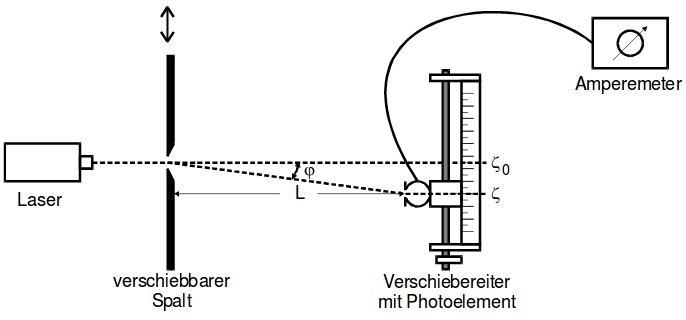
\includegraphics[scale=0.4]{aufbau.png}
  \caption{Versuchsaufbau \cite{anleitung}.}
  \label{abb:4}
\end{figure}
\subsection{Versuchsdurchführung}
In einem vorbereitenden Schritt muss der Dunkelstrom am Photoelement gemessen werden.
Als Dunkelstrom bezeichnet man das durch das Restlicht des Abgedunkelten Raums auf das
Photoelement einfallende Licht. Dann werden die Beugungsbilder eins Einzelspalts
sowie zwei verschiedener Doppelspalte vermessen. Beim Einzelspalt werden neben dem
Hauptmaximum zusätzlich die Nebenmaxima 1. Ordnung gemessen, bei den Doppelspalten
die Nebenmaxima bis zur 2. Ordnung. Der Messbereich des Amperemeters wird dabei
nach Bedarf angepasst.
\section{Auswertung}
\subsection{Konstanten.}
Es wurde ein Helium-Neon-Laser mit einer Wellenlänge von \SI{635}{\nano\meter} verwendet.
Der Abstand zwischen Spalt und Photoelement beträgt \SI{125}{\centi\meter}. Außerdem wurde
ein Dunkelstrom von \SI{2}{\nano\meter} gemessen, der von allen Intensitäten abgezogen wurde.
\subsection{Beugung am Einzelspalt.}
\label{sec:einzel}
Bei der Regression wird \eqref{eq:4} mit Näherung \eqref{eq:6} als Funktion zur Grunde gelegt. Die zu fittenden Parameter
sind $A_0, b$ und $c$. Dabei ist $A_0$ die maximale Intensität, $b$ die Spaltbreite und
$c$ der x-Wert des Maximums. Es ergeben sich folgende Werte, die in Tabelle \ref{tab:1} dargestellt sind.
\begin{table}
  \centering
  \begin{tabular}{c c c}
    \toprule
    & Werte aus der Regression & Erwartete Werte \\
    \midrule
    $b$ & \SI{0.0747(6)}{\milli\meter} & \SI{0.075}{\milli\meter} \\
    $A_0$ & \SI{216.1(15)}{\nano\ampere} & \SI{260}{\nano\ampere} \\
    $c$ & \SI{25.494(31)}{\milli\meter} & \SI{25}{\milli\meter} \\
    \bottomrule
  \end{tabular}
  \caption{Parameter aus der Regression zum Einzelspalt.}
  \label{tab:1}
\end{table}
In Abbildung \ref{fig:1} ist die Regression mit den Messwerten grafisch dargestellt.
\begin{figure}
  \centering
  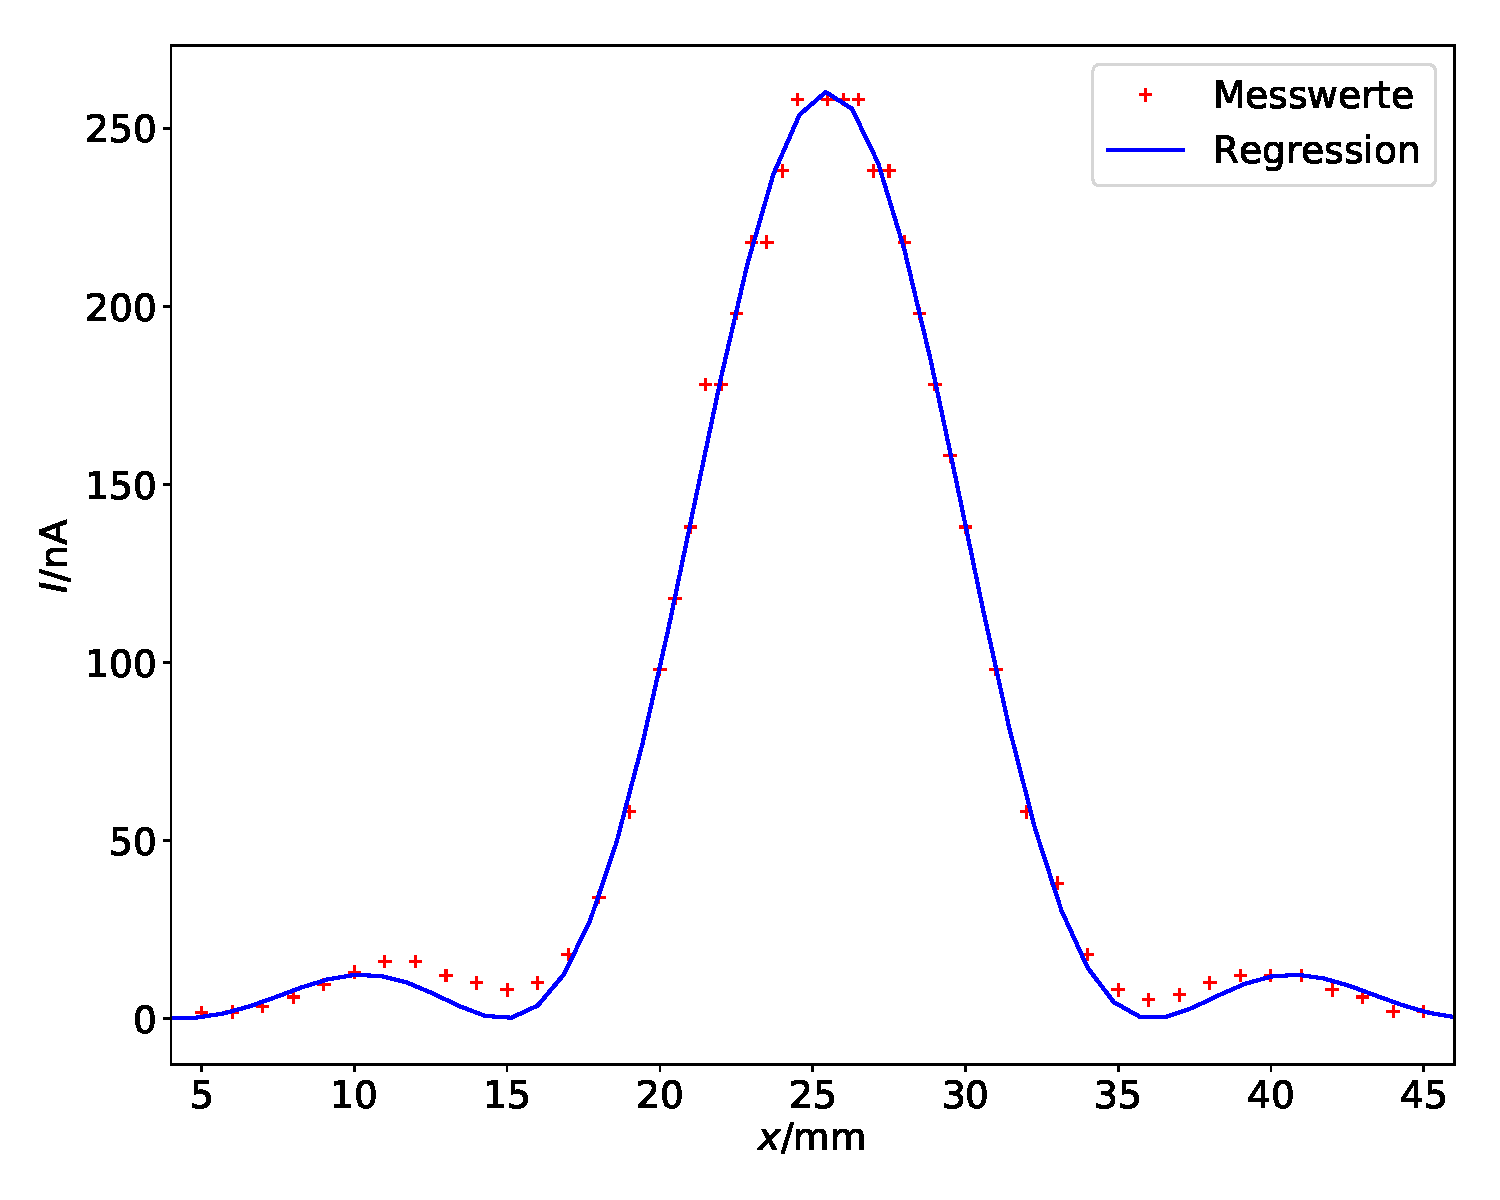
\includegraphics[scale=0.3]{einzel.pdf}
  \caption{Regression am Einzelspalt grafisch dargestellt.}
  \label{fig:1}
\end{figure}
\subsection{Beugung am ersten Doppelspalt.}
\label{sec:erster}
Für die Regression am Doppelspalt wird \eqref{eq:5} mit Näherung \eqref{eq:6} verwendet.
Die Fitparameter sind die gleichen wie in Kapitel \ref{sec:einzel}. Diese werden noch erweitert
durch die Gitterkonstante $s$. Die Ergebnisse der Regression sind in Tabelle \ref{tab:2} dargestellt.
\begin{table}
  \centering
  \begin{tabular}{c c c}
    \toprule
    & Werte aus der Regression & Erwartete Werte \\
    \midrule
    $b$ & \SI{0.1518(33)}{\milli\meter} & \SI{0.15}{\milli\meter} \\
    $A_0$ & \SI{4.86(12)}{\micro\ampere} & \SI{4.498}{\micro\ampere} \\
    $c$ & \SI{25.052(18)}{\milli\meter} & \SI{25}{\milli\meter} \\
    $s$ & \SI{0.2361(35)}{\milli\meter} & \SI{0.25}{\milli\meter} \\
    \bottomrule
  \end{tabular}
  \caption{Fitparameter aus der Regression \eqref{eq:5} für den ersten Doppelspalt mit den erwarteten Werten.}
  \label{tab:2}
\end{table}
Die grafische Darstellung ist in Abbildung \eqref{fig:2} zu finden.
\begin{figure}[h]
  \centering
  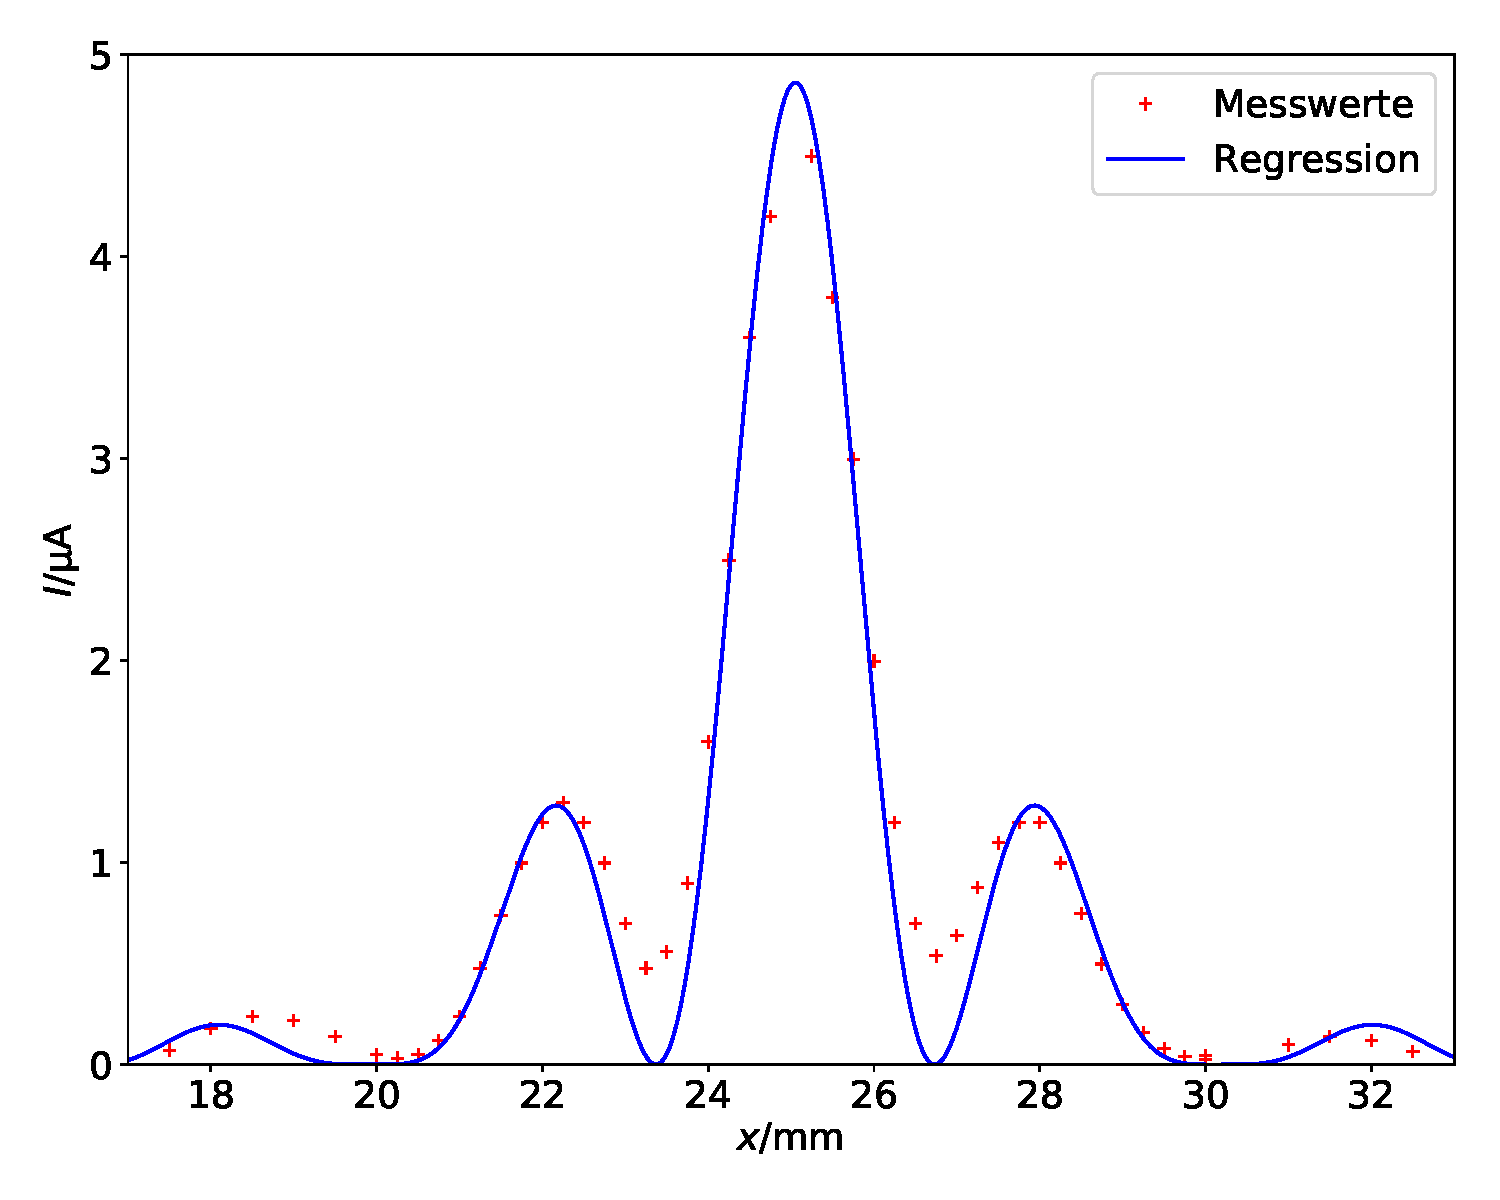
\includegraphics[scale=0.3]{doppelk.pdf}
  \caption{Grafische Darstellung der Regression am ersten Doppelspalt.}
  \label{fig:2}
\end{figure}
\subsection{Beugung am zweiten Doppelspalt.}
Die Vorgehensweise ist deckungsgleich mit der aus Kapitel \ref{sec:erster}. Die Ergebnisse
sind in Tabelle \ref{tab:3} dargestellt. Die grafische Darstellung findet sich in Abbildung \ref{fig:3}.
\begin{table}[h]
  \centering
  \begin{tabular}{c c c}
    \toprule
    & Werte aus der Regression & Erwartete Werte \\
    \midrule
    $b$ & \SI{0.155(11)}{\milli\meter} & \SI{0.15}{\milli\meter} \\
    $A_0$ & \SI{9.3(7)}{\micro\ampere} & \SI{7.398}{\micro\ampere} \\
    $c$ & \SI{25.076(25)}{\milli\meter} & \SI{25}{\milli\meter} \\
    $s$ & \SI{0.483(9)}{\milli\meter} & \SI{0.5}{\milli\meter} \\
    \bottomrule
  \end{tabular}
  \caption{Fitparameter aus der Regression \eqref{eq:5} für den zweiten Doppelspalt mit den erwarteten Werten.}
  \label{tab:3}
\end{table}
\begin{figure}
  \centering
  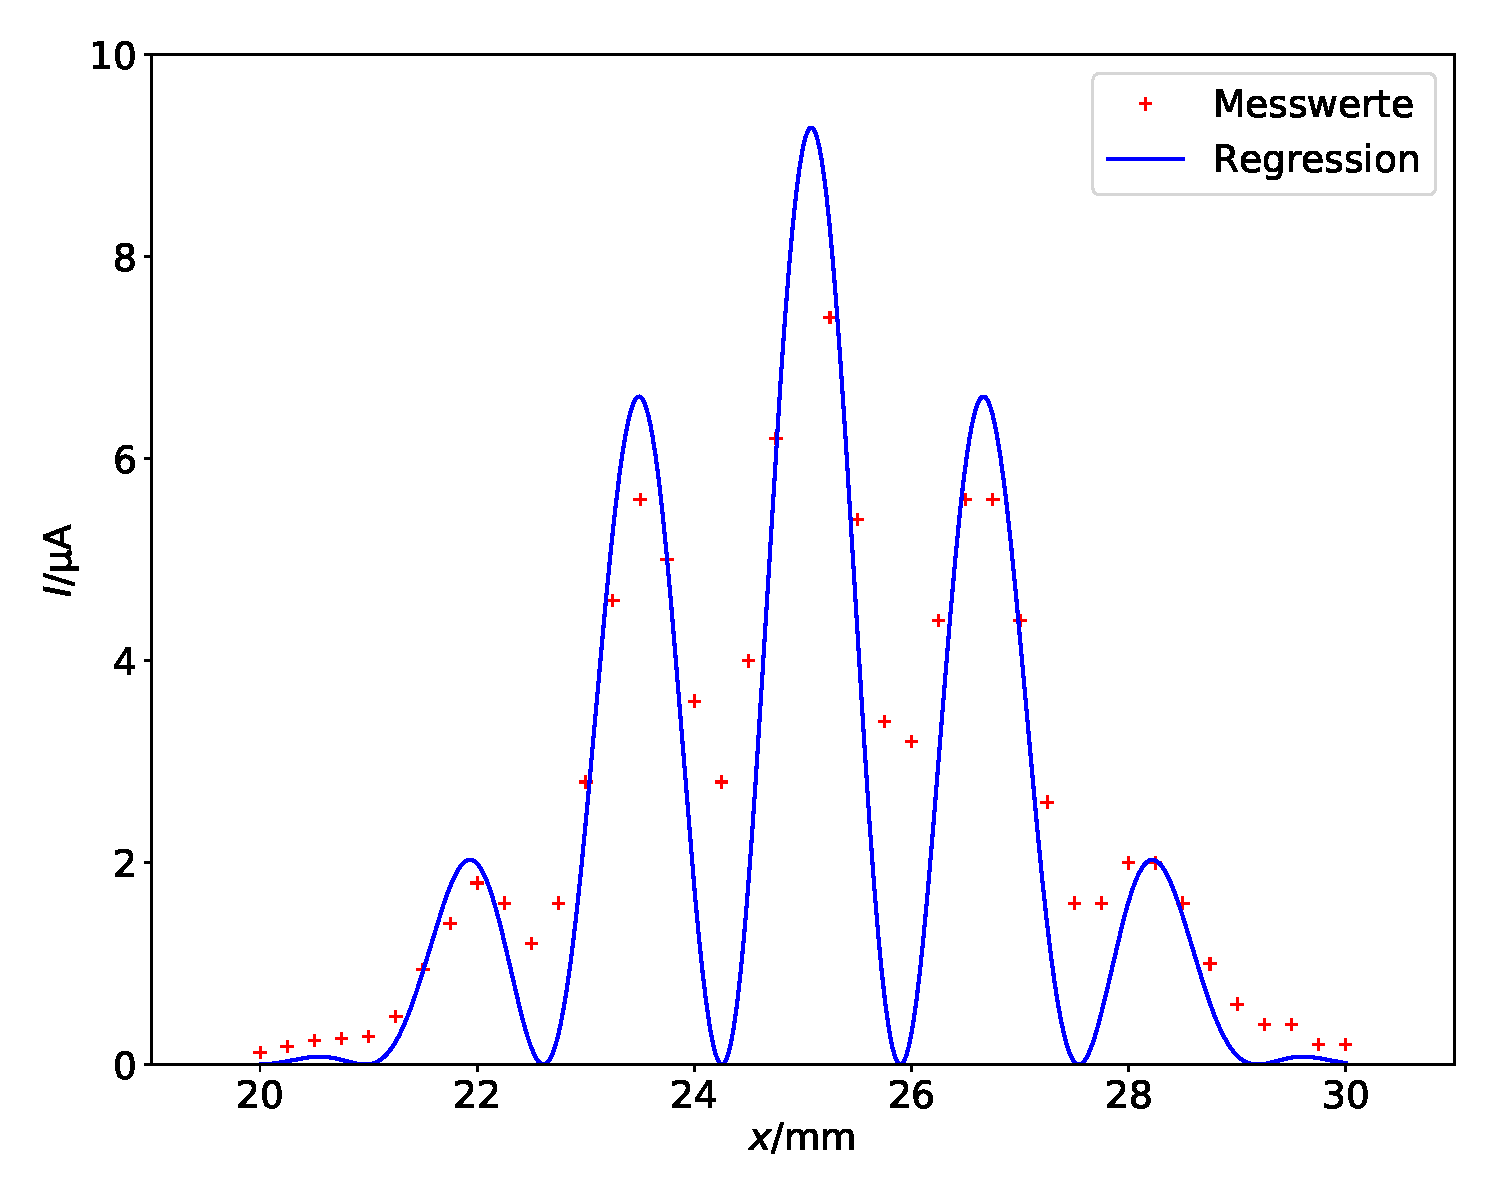
\includegraphics[scale=0.3]{doppelg.pdf}
  \caption{Grafische Darstellung der Regression am zweiten Doppelspalt.}
  \label{fig:3}
\end{figure}


\section{Diskussion}
Zur Beugung am Einzelspalt lässt sich sagen, dass alle gefitteten Parameter in der
Messungenauigkeit liegen (siehe Tabelle \ref{tab:1}). An Abbildung \ref{fig:1} lässt sich erkennen, dass sich die Messwerte
gut an die Regression anpassen. Abschließend lässt sich zu diesem Versuchsteil also sagen, dass
die Methode gute Werte geliefert hat. \\
\\
Die Beugung an den beiden Doppelspalten hat gute Ergebnisse geliefert (siehe Tabellen \ref{tab:2} und \ref{tab:3}).
Die erwartete Spaltbreite $b$ beim ersten Doppelspalt liegt innerhalb der Messungenauigkeit,
die anderen Parameter liegen in der gleichen Größenordnung und haben geringe relative Abweichungen,
zum Beispiel 5,6\% bei der ersten Gitterkonstante. Aus den Plots wird deutlich, dass der gefittete Wert von $A_0$
gut zum tatsächlichen Maximum der Regression passt. Die Abweichung zum erwarteten Wert kommt daher,
dass dieser lediglich das Maximum der Messwerte und nicht das globale Maximum darstellt. Außerdem
wird ersichtlich, dass bei einer höheren Gitterkonstante mehr Nebenminima und engere und höhere Hauptmaxima
auftreten. Weiterhin wird aus den Abbildungen \ref{fig:2} und \ref{fig:3}
deutlich, dass vor allem bei den ersten beiden Nebenminima zu wenige Messwerte vorhanden sind,
um die Regression gut anzunähern. Vor allem beim zweiten Doppelspalt würde man mit mehr Messwerten
eine bessere Näherung erhalten.
\newpage
\nocite{*}
\printbibliography
